\section{System Design}
\label{sect:arch}


%\begin{figure}[htbp]
%  \centering
  %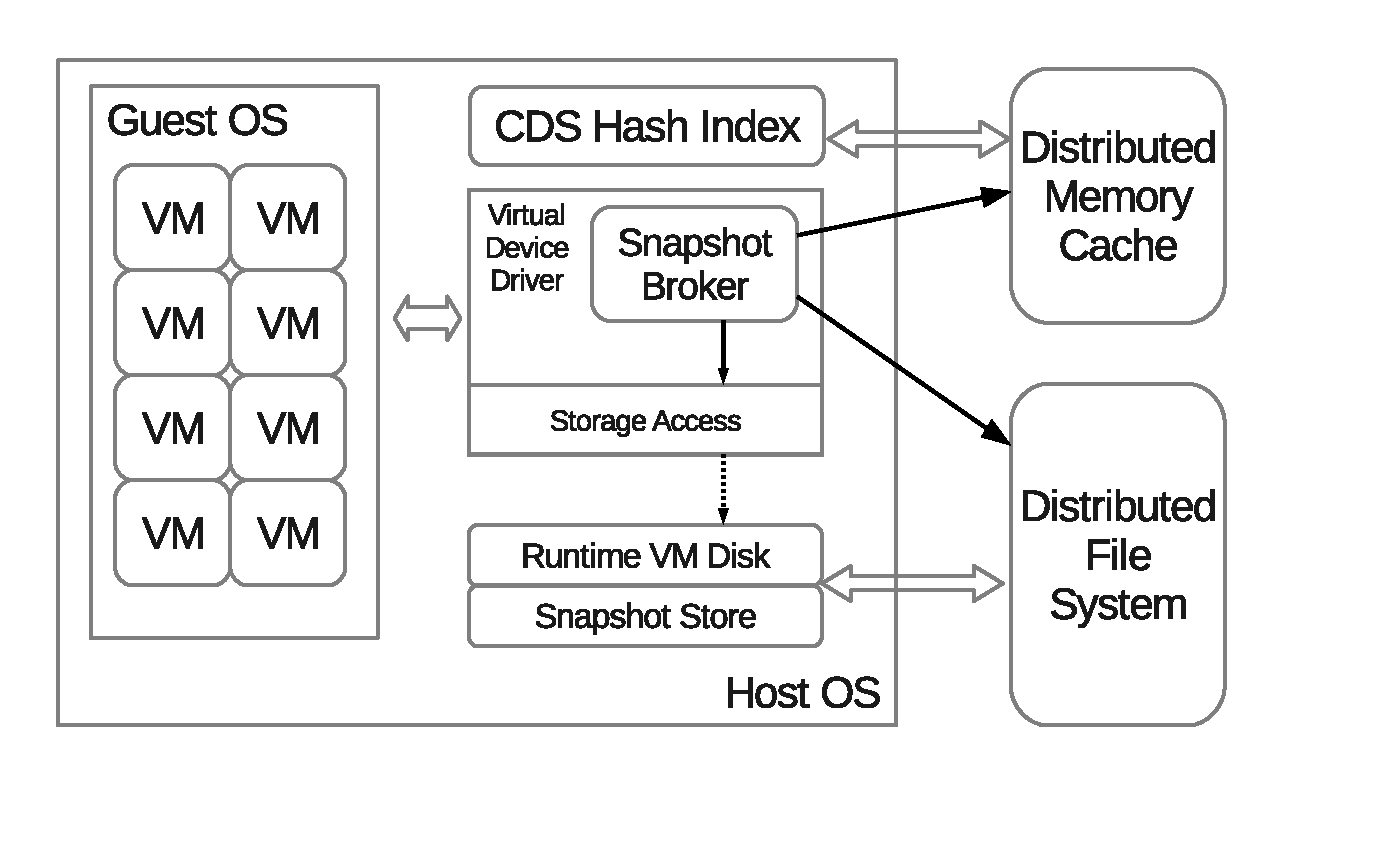
\epsfig{file=images/arch.eps, height=2in, width=2.66in}
%  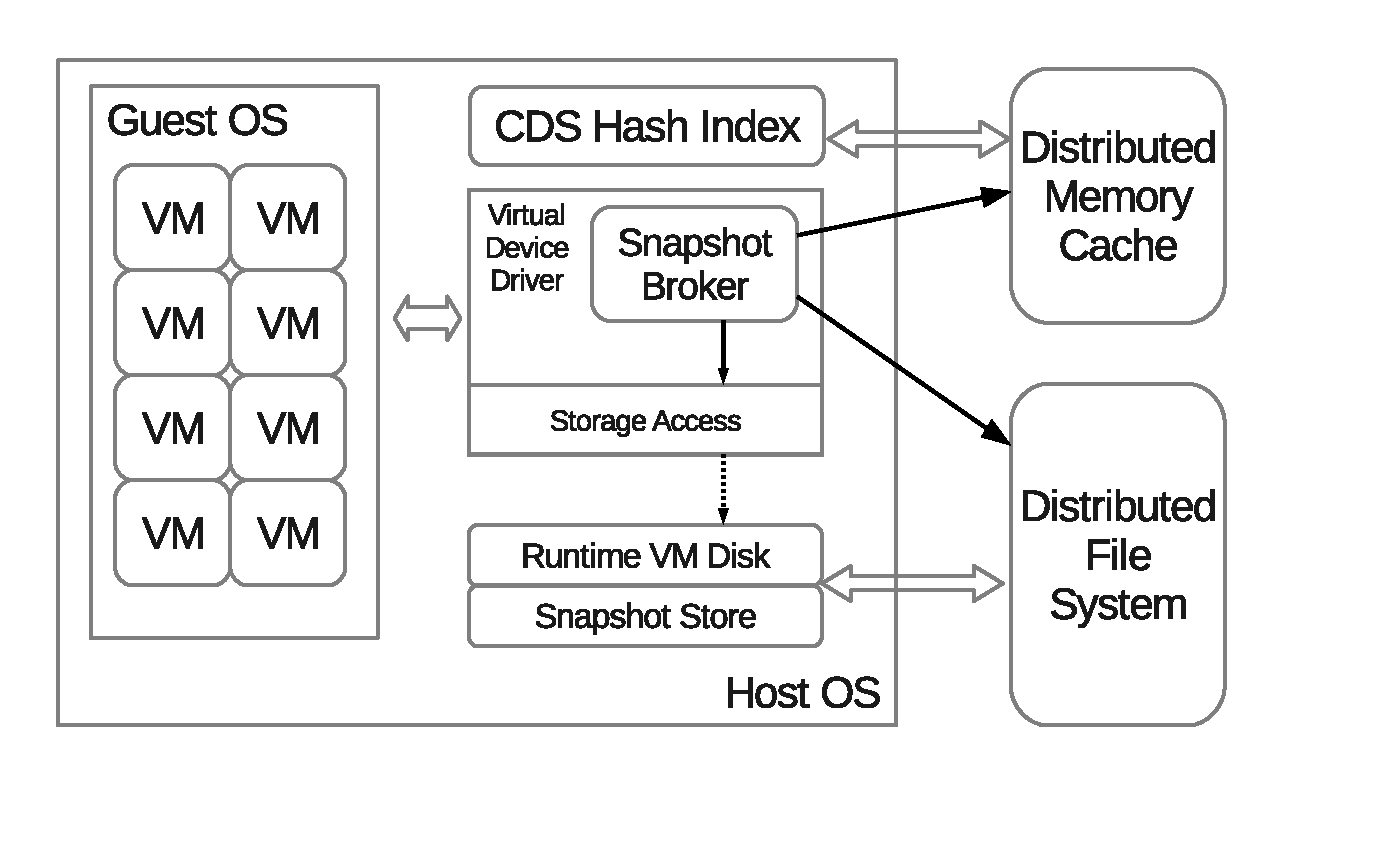
\epsfig{file=images/arch.eps, width=3.9in}
%  \caption{Snapshot backup architecture of each node.}
%  \label{fig:arch}
%\end{figure}



We consider deduplication in two levels. The first level
uses coarse-grain segment  dirty bits for version-based detection~\cite{Clements2009,Vrable2009}.
% to identify difference from the previous snapshot to the current snapshot.  
%That  can be accomplished efficiently and inexpensively in the OS level.
%We use a segment-level coarse-grain setting to reduce the efforts in detection and maintaining dirty bits. 
Our experiment with Alibaba's production dataset shows that over 70 percentage of 
duplicates can be detected using segment dirty bits when the segment size is 2M bytes.  
This setting requires the virtual disk driver to maintain segment dirty bits,
which has a negligible space cost (1 bit per 2 MB). In the second level of deduplication, content blocks of dirty segments 
are compared with the fingerprints of unique  blocks from previous snapshots.
Our key strategies are explained as follows.
\begin{itemize}


\item {\bf Separation of duplicate detection and data backup.}
%Request accumulation and partition-based deduplication.}
The second level detection requires a global comparison of fingerprints.
% of stored chunks with the new chunks scanned during the backup process. 
%Bloom filters and caching allows some of content 
%fingerprints to be stored on the cheap disks~\cite{bottleneck08}. Such an optimization is good 
%for inline deduplication where chunks scanned need to be determined to be duplicate or not instantly without 
%waiting while  it memory consumption is still significant in competing with stand virtual 
%machine activities.  
Our approach is to perform duplicate detection first before actual data backup.
That requires a prescanning of  dirty VM segments, which
%  and after that, real backup  for those non-duplicates is conducted. 
does incur an extra  round of VM reading.
% while avoiding inline deduplication and leading to a much smaller resource requirement.  
During VM prescanning, detection requests are accumulated.
Aggregated deduplicate requests can be processed partition by partition. 
%We also accumulate the delete requests and perform them partition by partitions. 
Since each partition corresponds to a small portion of global index, 
memory cost to process detection requests within a partition is small.
%the cost to process detection requests within a partition is significantly smaller than processing all 
%the requests globally.

\item {\bf Buffered data redistribution in parallel duplicate detection}.  
Let {\em global index} be the meta data containing the fingerprint values of unique snapshot blocks 
in all VMs and  the reference pointers to the location of raw data.
%A duplicate detection request for a content block needs to be compared with the global index to determine if this
%block is non-duplicate. If it is a duplicate, return the corresponding reference pointer.
%We conduct parallel processing of detection requests in all machines involved. 
A logical way to distribute detection requests among machines is based on 
fingerprint values of content blocks.
% in a  disjointed manner.
Initial data  blocks follow the VM distribution 
among machines 
and the detected duplicate summary 
should be collected following the same distribution.
Therefore, there are four all-to-all data redistribution operations involved.
One is to map detection requests from VM-based distribution to fingerprint based distribution, and
another one  is to map duplicate summary from fingerprint-based distribution to VM based distribution.
Two additional rounds are required to ensure no duplicate blocks are missed
and that both the partition index holder and VM owning machines have correct
data references.
The redistributed data needs to be accumulated on the disk to reduce the use of memory.
To minimize the disk seek cost, outgoing or incoming data exchange messages are buffered to 
bundle small messages.
Given there are $p\times q$ partitions where $p$ is the number of machines and $q$ is the number of fingerprint-based partitions
at each machine, space per each buffer  is small under the memory constraint for large $p$ or $q$ values.
This counteracts the effort of seek cost reduction.  
%Then there will be a large number of storage  IO operations involved, suffering the huge seek overhead.
We have designed an efficient data exchange and disk data buffering  scheme to address this.
\item {\bf Round Scheduling}.
When all data is scheduled to be deduplicated in one round, the cost of Copy
on Write (CoW) can be significant, as explored in other papers\cite{EMCIncrementalDataChanges}.
We therefore develop an algorithm to break up the data into multiple rounds to
make the best use of the efficiency of batch processing, while minimizing
the cost of CoW.

%As we detect and backup requests before actual backup takes place,  we need to store chunk data on 
%temporary disks and once duplicates 
%are detected, we only need to fetch and store these non-duplicates 
%in the backup storage.  To minimize the storage usage of temporary disk space, we donot save the data content 
%of accumulated requests with replication, but we store  data separately for each virtual machine. In an event 
%that the storage of temporary accumulation fails for certain virtual machines, rescanning of these virtual machine images 
%is conducted and backup of these machines is re-initiated.   Meta data such as content hash for accumulated requests 
%is stored separately since we map the meta data into a set of buckets using chunk fingerprints. 
%The benefit of separating content and meta data is to allow fast recovery of backup operations while enabling bucket-based lazy deduplication.

\end{itemize}


We assume a flat architecture in which  all $p$ machines that host VMs in a cluster can 
be used in parallel for deduplication. 
A small amount of local disk space and memory on each machine can be used 
to store global index and temporary data. 
The real backup storage can be either a distributed file system built on
this cluster  or use another  external storage system. 
%Our design is to minimize the usage of local memory and storage on each machine.


%While we assume all machines can process  independent or coordinated
%deduplication and backup operations in parallel,  
%our scheme uses a single-thread procedure on each machine to minimize the use of CPU, network bandwidth, and disk bandwidth.

\begin{figure}
\centering
\includegraphics[width=0.5\textwidth]{images/batch_arch.pdf}
\caption{Overall architecture of parallel VM snapshot deduplication}
\label{fig:snapshot}
\end{figure}
%\subsection{Snapshot Representation}

The representation of each snapshot in the backup storage
has a two-level index structure in the form of a hierarchical
directed acyclic graph.% as shown in Figure~\ref{fig:snapshot}.
A VM image is divided into a set of segments and each  segment contains 
content blocks of variable-size, partitioned using
the standard chunking technique with 4KB as the average block size. 
%the standard chunking technique~\cite{similar94} with 4KB as the average block size. 
%To simplify the deduplication process, segments are aligned to fix-sized boundaries, currently using 2MB.
The snapshot metadata  contains a list of segments and other meta data information.
Segment metadata  contains its  content block fingerprints and reference pointers. 
If a segment is not changed from one snapshot to another, indicated by a dirty bit embedded in the virtual disk driver, 
%its content blocks are not changed as well, thus 
its segment metadata contains a reference pointer to an earlier segment.
For a dirty segment, if one of its blocks is duplicate to another block in the system,  
the block metadata contains a reference pointer to the earlier block.





%\begin{figure*}[tbhp]
%\centering
%\includegraphics[width=0.95\textwidth]{images/DataFlow.pdf}
%\caption{Processing flow of Stage  1 (dirty segment scan and request accumulation), Stage 2 
%(fingerprint comparison and summary output),  and Stage 3 (non-duplicate block backup).}
%\label{fig:flow}
%\end{figure*}

\begin{figure}[th]
\centering
\includegraphics[width=0.5\textwidth]{images/Stage1.pdf}
\caption{Processing flow of Stage 1.}
\label{fig:stage1}
\end{figure}

%\subsection{Processing flow and resource usage}
%The data flow of our multi-stage duplicate detection is depicted in Figure~\ref{fig:flow}. 
%\begin{itemize}
%\item
In Stage 1a, each machine independently reads  
%$v/k$  
VM images that need a backup
and forms duplicate  detection requests. 
%For those dirty segments,
%segments that have been modified since last backup indicated by dirty bits,  
The system divides  each dirty segment into a sequence of chunk blocks,  computes the meta 
information such as chunk fingerprints,  sends a request to a proper machine, and accumulates  
received requests into a partition on the local temporary disk storage. 
The partition mapping uses a hash function applied to the content fingerprint. 
Assuming all machines have a  homogeneous resource configuration, each machine is evenly  assigned with
$q$ partitions of global index and it accumulates corresponding requests on the disk. 
There are two options to allocate buffers at each machine. 
1) Each machine has  $p\times q$ send buffers corresponding to $p\times q$ partitions in the cluster
since a content block in a VM image of this machine can be sent to any of these partitions.
2) Each machine allocates $p$ send buffers to deliver requests to $p$ machines; it allocates 
$p$ receive buffers to collect requests  from other machines.
Then the system copies requests from each of $p$ receive buffers to  $q$ local request buffers,
and outputs each request buffer to one of the request partitions on the disk
when this request buffer becomes full.  Option 2, which is  depicted in Figure~\ref{fig:flow},
is much more efficient than Option 1 because $2p+q$ is much smaller than
$p\times q$, except for the very small  values. 
As a result, each buffer in Option 2 has a bigger size to accumulate requests and that means
less disk seek overhead.

%We assume that the startup cost for network message sending is  much more less (e.g. an order of magnitude
%less) than from one machine to another 
%disk storage startup cost such as seek is much mu
%Note that we only accumulate requests with their meta data information.
%\item
Stage 1b is to load disk data and perform fingerprint comparison at each machine one request partition at a time.
% in the partitions.  
%The system maintains the index of all chunk fingerprints divided in the buckets. 
%The system loads the global index partition 
%and accumulated corresponding requests, and compare them to  identify the duplicated blocks.  
%Then we unload them, load the global index and accumulated requests for another partition. 
%This process is repeated until all buckets are processed.
At each iteration, once in-memory comparison between an index partition and request partition is completed,  
duplicate summary information for segments of each VM is routed from the fingerprint-based distribution  to the
VM-based distribution.  The summary contains the block ID and  the reference pointer for each detected duplicate block.   
Each machine uses memory space of the request partition as a send buffer with no extra memory requirement.
But it needs to allocate $p$ receive buffers to collect duplicate summary from other machines.
It also allocates $v$ request buffers to copy duplicate summary from $p$ receive buffers and output to the local disk
when request buffers are full. One potential issue is that there may be
multiple copies of a new block added to the system during the same round.
We call these dup-with-new blocks and the redundandy is discovered and
logged during the index lookup.
Our experience is that there is significant redundancy during the initial snapshot backup and after
that, the percentage of redundant blocks due to concurrent processing  is small.

\begin{figure}[th]
\centering
\includegraphics[width=0.5\textwidth]{images/Stage2.pdf}
\caption{Processing flow of Stage 2.}
\label{fig:stage2}
\end{figure}

In stage 2a the deduplication results corresponding to unique (new) data blocks
are exchanged using $p$ send and receive buffers to route the responses to the
deduplication requesters. Dup-with-new blocks are not exchanged, as they are
treated as duplicate blocks, only without data references (the data references
to these blocks are added in Stage 3).

%. In this way, it sends duplicate summary to the corresponding machines one by one to minimize the startup cost for sending a message.
%In the receiving side, 
%All-to-all machines data exchange is conducted  so that  
%each machine allocates $q$ receive buffers corresponding to
%$q$ local partitions, to hold received messages from other machines.  
%When a receive buffer for a VM is  full, the data is written to the local disk storage. 
%These substeps are repeated as the stream of data is exchanged when each machine compares through all $q$ partitions.

%\item 
Stage 2b is to perform the real backup.
% one VM at a time.
The system loads the duplicate summary of a VM, 
reads  dirty segments of a VM, and outputs non-duplicate blocks to the final backup 
storage. Additionally, references to each new data block are saved so that the
global index may be updated.%the global index on each machine is updated with the meta data of new chunk blocks. 
When a segment is not dirty, the system only needs to output the segment meta data such as a reference pointer. 
There is an option to directly read dirty blocks instead of fetching a dirty segment which can include duplicate
blocks. Our experiment shows that it is faster to read dirty segments in the tested workload.
%Another issue is that during global index update after new block creation,
% in the backup storage,
%the system  may find some  blocks with the same fingerprints have been 
%created redundantly. For example, two different VM blocks that have the same  fingerprint are not detected
%because  the  global index has not contained such a fingerprint yet. 

%If a segment is dirty,  the system  use the duplicate summary information from Step 2 for internal 
%duplicate blocks of this dirty segment and output the remaining non-duplicate blocks to the backup storage.
%\end{itemize}

%          In fetching non-duplicates,    it is sometime faster that we fetch a large number of consecutive chunk blocks from an accumulated  segment which contains duplicated chunks,  to avoid the random seek overhead.

\begin{figure}[th]
\centering
\includegraphics[width=0.5\textwidth]{images/Stage3.pdf}
\caption{Processing flow of Stage 3.}
\label{fig:stage3}
\end{figure}

In Stage 3a the machines exchange references to new blocks. This is required
because it is the VM holder that backs up the data, but the partition index
holder that must perform index lookups. Each machine reads the references
obtained for all new blocks written, and then sends those references to the
partition index holder, and the received references are saved to disk during 3a.

Stage 3b is where the index update occurs; new blocks are added to each
partition index, and additionally dup-with-new blocks are re-read to obtain
references. The dup-with-new blocks, now with references, are added to the
duplicate result lists to be returned in Stage 4.

\begin{figure}[th]
\centering
\includegraphics[width=0.5\textwidth]{images/Stage4.pdf}
\caption{Processing flow of Stage 4.}
\label{fig:stage4}
\end{figure}

In the final Stage of our algorithm, Stage 4, All duplicate references,
including dup-with-new blocks, are returned to the requesters from the index
holders and the snapshot
recipes are updated with those pointers.


The above steps can be executed by each machine using one thread to minimize
the use of computing resources.
The  disk storage usage on each machine 
is fairly small for  storing part of the global index and
accumulating  duplicate detection requests that contain fingerprint information.   
We impose a memory limit $M$ allocated for each stage of processing at each machine.
%The usage of $M$ is controlled as follows and space allocation among buffers is optimized based on the relative
%ratio between the cross-machine network  startup cost and disk access startup cost such as seek time.
%Using a bigger buffer  can mitigate the impact of slower startup cost. 
$M$ includes space for network communications and buffering data which is being
sent to disk. We have found that as long as the write/read buffers are not
unreasonably small (e.g. 4KB), the size of the disk buffers does not have a
great impact on backup time, so we allocate small disk buffers (e.g. 128KB read
and 2.5MB shared across all write buffers), and then allocate the remaining
memory to index space or network buffers, depending on the stage.
\begin{itemize}
\item For Stage 1, $M$ is divided for 
1) an I/O buffer to read dirty segments; 2) $2p$ send/receive buffers and $q$
disk buffers for deduplication requests.

%1) $p$ send buffers. images, sends the fingerprint of a dirty block to a machine that is responsible for this fingerprint.
%2) Buffer requests gathered from other machines and divide those requests into $q$ buckets. Once a buffer for each bucket is full, output to the disk storage.
\item 
For Stage 2, $M$ is divided for 1) space for hosting a global index partition and 
the corresponding request partition; 2) $p$ receive buffers and $v$ summary buffers.
%%accumulating duplicate summary for each targeted VM.   Once  each machine processes a bucket of  duplicate detection requests, 
%For each machine which hosts $v$  VMs, and will receive messages from many other machines, 
%the system needs to allocate buffer space for each VM ot accumulate the duplicate summary records. 
%When a buffer for a VM is full, the result is written to the disk.

\item For Stage 3, $M$  is divided for 1) an I/O buffer to read dirty segments of a VM and   
write non-duplicate blocks to the  backup storage;
2) summary of duplicate blocks within dirty segments. 
\end{itemize}
%We find the memory for step 2 is most critical for buffering duplicate summary in hiding the latency. 
%Certainly most storage system can allow many IO requests issued in parallel overlapping the IO latency.  
%Here we assume the worst case and also minimize the IO bandwidth usages by issuing 
%one request at a time to use the minimal disk bandwidth resource.

{\bf Snapshot deletion.} Each VM will keep a limited number of  automatically-saved snapshots and 
expired snapshots are normally deleted.
% unless its owner explicitly asks for its retention.
We adopt the idea of mark-and-sweep~\cite{Guo2011}. 
A block or a segment can be deleted if its reference count is zero.
%As we discussed in Section~\ref{sect:data}, the reference counter is kept in the global index, partitioned among machines. 
To delete useless  blocks or segments periodically, we read the meta data  of all
snapshots and compute the reference count of all blocks and segments  in parallel.
%while following the fingerprint-based partitioning.
Similar to the multi-stage duplicate detection process, reference counting is conducted in multi-stages. 
Stage  1 is to read  the segment and block  metadata 
to accumulate  reference count requests in different machines  in the fingerprint based distribution.
Stage   2 is to count references within each partition and detect those records with zero 
reference. 
%Stage 3 is that every VM gathers its z confirmed deletion requests for its content and sends them to the backup storage.
The backup  data repository logs deletion instructions,  and will periodically perform a compaction operation when 
its deletion log is too big. 
%Due to the paper constraint, we will not discuss the deletion operations in details.

%The above method requires the counter information to be consistently maintained in the global index.
%Finally the deleteion summary. it will adjust the corresponding reference counts. At the end of bucket worker's operation, it outputs the unused blocks information to each VM data repository's deletion log.


%This compaction will make a copy of all the data in use, and remove the obsoleted blocks. However, after such a compaction, many block offsets will be changed, as a result, such changes are sent to the bucket job queue so that changes will be reflected upon the next bucket update.

%Since we maintain a single copy of each block information in the bucket index, and there is at most one bucket worker operating the bucket index at one time, it it safe to do the simple referencec ounting rather than mark-and-sweep.
